% by Ohce Qin
%Using TeX Live 2014 and WinEdt 9.0
%Compile with PDFLaTeX Version 3.14159265-2.6-0.99991
% 2015-04
%qinyc@hotmail.com
%%%%%%%%%%%%%%%%%%%%%%%%%%%%%%%%%%
%in 2016 updated by Chicken John
%Using MikTeX and Texmaker
%Compile with XeLaTeX Version 3.14159265-2.3-0.99975
% 2016-01
%chickenjohn93@outlook.com

\documentclass[12pt,a4paper]{article}
%\usepackage{ctex}
%\usepackage[center]{titlesec}%章节标题位置
\usepackage[BoldFont,SlantFont,CJKsetspaces,CJKchecksingle]{xeCJK}
\usepackage{amsmath}
\usepackage{amsfonts}
\usepackage{bm}%bold form in math environment
 %\sideset{}{}\sum  求和符号左上角,右上角添加标记
\usepackage{graphicx}
\usepackage{wrapfig}
\usepackage{subfigure}%多图共用caption
%\usepackage[version=3]{mhchem} %化学式  \ce{*} 见数字均为下标
\usepackage[CJKbookmarks,bookmarksnumbered,
                     bookmarksopen,colorlinks,citecolor=blue,
                     linkcolor=blue]{hyperref}%链接样式
\usepackage{geometry}
\usepackage{fontspec,xunicode,xltxtra}
\usepackage{titlesec}
\usepackage{indentfirst}
\usepackage{multicol}
\usepackage{amssymb}
\usepackage{amsthm}
%\usepackage{mathabx}
\usepackage{multirow}
\usepackage{diagbox}
%\usepackage{fixltx2e}%解决caption中使用向量的问题配合命令\MakeRobust{\overrightarrow}
%\usepackage{exercise}
\usepackage{fancyhdr}
\usepackage{titling}%调整title
\usepackage{tabu,tikz}
\usepackage{setspace} 
\usepackage{textcomp} %support other codes
\usepackage{listings} %codes support
\usepackage{xcolor}
\usepackage{pdfpages} %insert pdf

%\usepackage{blindtext}%?
%\usepackage[svgnames]{xcolor} % Required to specify font color

\XeTeXlinebreaklocale "zh"
%\XeTeXlinebreakskip = 0pt plus 1pt minus 0.1pt
\geometry{top=10mm,bottom=10mm,left=20mm,right=20mm}%调整正文上下边距
\renewcommand{\headrulewidth}{0pt}  %页眉线宽,设为0可以去页眉线
\lhead{}%页眉左边
\rhead{}%页眉右边
%\oddsidemargin=11mm
%\evensidemargin=5mm
\setCJKmainfont{SimSun}
\setCJKmonofont{SimSun}
\setmainfont{Times New Roman}
\fontsize{10.5pt}{15.7pt}\selectfont
\graphicspath{{Titlepage/}{Sect1/}{Sect2/}{Sect3/}{Sect4/}}
%\numberwithin{equation}{section}

\pagestyle{fancy}
%-------调整表格线条粗细-------
%\newcolumntype{L}[1]{>{\vspace{0.5em}\begin{minipage}{#1}\raggedright\let\newline\\
%\arraybackslash\hspace{0pt}}m{#1}<{\end{minipage}\vspace{0.5em}}}
%\newcolumntype{R}[1]{>{\vspace{0.5em}\begin{minipage}{#1}\raggedleft\let\newline\\
%\arraybackslash\hspace{0pt}}m{#1}<{\end{minipage}\vspace{0.5em}}}
%\newcolumntype{C}[1]{>{\vspace{0.5em}\begin{minipage}{#1}\centering\let\newline\\
%\arraybackslash\hspace{0pt}}m{#1}<{\end{minipage}\vspace{0.5em}}}
%\makeatletter
%\def\hlinewd#1{%
%  \noalign{\ifnum0=`}\fi\hrule \@height #1 \futurelet
%   \reserved@a\@xhline}
%\makeatother
%--------------------------------

% \def\degree{${}^{\circ}$}
% \def\ee{\mathrm{e}}%自然对数底数
% \def\ii{\mathrm{i}}%复数单位
% \def\dd{\mathrm{d}}
% \def\pp{\partial}
% \def\z{\left}
% \def\y{\right}
% \def\ol{\overline}
% \def\ora{$\overrightarrow{}$}

%----------字体相关----------
\setCJKfamilyfont{song}{SimSun}
\newcommand{\song}{\CJKfamily{song}} 
\setCJKfamilyfont{hei}{SimHei}
\newcommand{\heiti}{\CJKfamily{hei}}
\setCJKfamilyfont{zs}{STZhongsong}
\newcommand{\zhongsong}{\CJKfamily{zs}}
\setCJKfamilyfont{kai}{KaiTi}
\newcommand{\kaishu}{\CJKfamily{kai}} 
\newfontfamily\Rom{Times New Roman}
\setCJKfamilyfont{xingkai}{STXINGKA.TTF}
\newcommand{\xingkai}{\CJKfamily{xingkai}}
\setlength{\baselineskip}{0em}
\newcommand{\chuhao}{\fontsize{42pt}{\baselineskip}\selectfont}     %初号  
\newcommand{\xiaochuhao}{\fontsize{36pt}{\baselineskip}\selectfont} %小初号  
\newcommand{\yihao}{\fontsize{28pt}{\baselineskip}\selectfont}      %一号  
\newcommand{\erhao}{\fontsize{21pt}{\baselineskip}\selectfont}      %二号  
\newcommand{\xiaoerhao}{\fontsize{18pt}{\baselineskip}\selectfont}  %小二号  
\newcommand{\sanhao}{\fontsize{15.75pt}{\baselineskip}\selectfont}  %三号  
\newcommand{\sihao}{\fontsize{14pt}{18pt}\selectfont}%     四号  
\newcommand{\xiaosihao}{\fontsize{12pt}{18pt}\selectfont}  %小四号  
\newcommand{\wuhao}{\fontsize{10.5pt}{15.7pt}\selectfont}    %五号  
\newcommand{\xiaowuhao}{\fontsize{9pt}{13pt}\selectfont}   %小五号  
\newcommand{\liuhao}{\fontsize{7.875pt}{\baselineskip}\selectfont}  %六号  
\newcommand{\qihao}{\fontsize{5.25pt}{\baselineskip}\selectfont}    %七

%\newcommand{\bb}[1]{\raisebox{-2ex}[0pt][0pt]{\shortstack{#1}}}% 表格中向下移动文字2ex
\renewcommand{\abstractname}{\xiaoerhao \heiti \textbf{摘~~要}}
\renewcommand{\contentsname}{\xiaoerhao \heiti \textbf{目~~录}}
\renewcommand{\figurename}{\wuhao\kaishu 图}
\renewcommand{\tablename}{\wuhao\kaishu 表}
\renewcommand\refname{\sihao \song \textbf{参考文献}}
%\renewcommand{\thesubsection}{\Alph{subsection}}
\titleformat{\section}{\sihao \song \bf}{\thesection}{1em}{}
\titleformat{\subsection}{\xiaosihao \song \bf}{\thesubsection}{1em}{}
%\MakeRobust{\overrightarrow}%解决caption中使用向量的问题配合命令\usepackage{fixltx2e}
%\MakeRobust{\vv}
%
%\makeatletter
\def\fnum@figure#1{\figurename\nobreakspace\thefigure\hspace{1em}}% 去掉图后面的冒号并加空白空1em
\def\fnum@table#1{\tablename\nobreakspace\thetable\hspace{1em}}% 去掉表后面的冒号并加空白1em
%\makeatother

\hypersetup{colorlinks=false,pdfborder=0 0 0} 
%\setcounter{tocdepth}{2}

%\setlength{\droptitle}{-4em}     % Eliminate the default vertical space
%\addtolength{\droptitle}{-20mm}



\begin{document}
%%%%%%%%%%%%%%%%%%%%%%%%%%%%%%%code support%%%%%%%%%%%%%%%%%%%%%%%%%%%%
\lstset{basicstyle=\fontsize{10.5pt}{9pt}\selectfont,breaklines=true,numbers=left,numberstyle=\tiny,keywordstyle=\color{blue!70},commentstyle=\color{red!50!green!50!blue!50},frame=shadowbox, rulesepcolor=\color{red!20!green!20!blue!20},escapeinside=``,xleftmargin=2em,xrightmargin=2em, aboveskip=1em}
%%%%%%%%%%%%%%%%%%%%%%%%%%%%%%%code support end%%%%%%%%%%%%%%%%%%%%%%%%
\input{Titlepage/title}
\thispagestyle{empty}
\begin{center} 
~~\\
\vspace{1cm}
\xiaoerhao
\heiti
\textbf{学位论文原创性声明}\\
\end{center}
\song
\fontsize{12pt}{24pt}\selectfont
~~\\
\indent 本人郑重声明:所呈交的论文是本人在导师的指导下独立进行研究所取得的研究成果。除了文中特别加以标注引用的内容外,本论文不包括任何其他个人或集体已经发表或撰写的成果作品。本人完全意识到本声明的法律后果由本人承担。\\
~~\\
\rightline{作者签名:~~~~~~~~~~年~~~~月~~~~日}

\begin{center}
~~\\
\vspace{1cm}
\xiaoerhao
\heiti
\textbf{学位论文版权使用授权书}\\
\end{center}
\song
\fontsize{12pt}{24pt}\selectfont
~~\\
\indent 本学位论文作者完全了解学校有关保障、使用学位论文的规定,同意学校保留并向有关学位论文管理部门或机构送交论文的复印件和电子版,允许论文被查阅和借阅。本人授权省级优秀学士论文评选机构将本学位论文的全部或部分内容编入有关数据进行检索,可以采用影印、缩印或扫描等复制手段保存和汇编本学位论文。\\
\indent 本学位论文属于 1、保密囗,在~~~~~~年解密后适用本授权书\\
\indent \phantom{aaaaaaaaaaaaaaa}2、不保密囗\\
\indent \phantom{aaaaaaaaaaaaaaa}(请在以上相应方框内打"√")
~~\\
\rightline{作者签名:~~~~~~~~~~年~~~~月~~~~日}
\rightline{导师签名:~~~~~~~~~~年~~~~月~~~~日}
\newpage
\setcounter{page}{1}
\begin{center}
\begin{table}
\begin{tabular}{|p{\columnwidth}|}
\hline
\sihao
\zhongsong
\vspace{0.1cm}
课题内容:\\
\song
\wuhao
\vspace{0.05cm}
~~~~~~毕业设计主要任务为:学习Android平台应用的开发,理解Activity、BroadcastReceiver、Content Provider和Service四个基本组件的属性与使用方法;学习TextView、SurfaceView、CardView等UI组件的使用方法;掌握Android平台与蓝牙模块之间建立通信、使用Socket接收数据的方法;掌握Android平台SQLite数据库操作方法;了解心电图(Electrocardiogram, ECG)各个导联的波形形态以及关键特征(如心率、RR间期、R峰峰值等);了解各个特征的测量方法;开发与蓝牙模块匹配的Android应用程序,使用UI组件实时显示ECG单个导联的波形;尝试在Octave平台实现ECG波形特征的提取算法,经过验证后在Android平台上实现;探究并实现一种有效的ECG数据显示方法。
\\
\\
\hline
\sihao
\zhongsong
\vspace{0.1cm}
课题任务要求:\\
\song
\wuhao
\begin{enumerate}
\setlength{\itemsep}{0pt}
\setlength{\parsep}{0pt}
\setlength{\parskip}{0pt}
\item 毕业设计选题;
\item 指导教师与学生见面,布置毕业设计任务;
\item 查阅相关中英文文献,制定毕业设计题目的实施方案、步骤,完成外文文献翻译、文献;
\item 文献阅读(开题报告)评阅、答辩、成绩评定;
\item 掌握Android Studio开发工具的使用;
\item 实现ECG波形特征的提取算法;
\item 实现Android的蓝牙通信,编写ECG波形显示应用程序;
\item 撰写毕业论文。
\end{enumerate}
\\ 
\hline
\sihao
\zhongsong
\vspace{0.1cm} 
主要参考文献\xingkai(由指导教师选定): \\
\song
\wuhao
\begin{enumerate}
\setlength{\itemsep}{0pt}
\setlength{\parsep}{0pt}
\setlength{\parskip}{0pt}
\item U. Satija, B. Ramkumar, and M. S. Manikandan. A simple method for detection and classification of ecg noises for wearable ecg monitoring devices. In Signal Processing and Integrated Networks (SPIN), 2015 2nd International Conference on, pages 164--169, Feb 2015.
\item Xiaoqiang Guo, Xiaohui Duan, Hongqiao Gao, Anpeng Huang, and Bingli Jiao. An ecg monitoring and alarming system based on android smart phone. Communications and Network, 05, 2013.
\item Dongdong Lou, Xianxiang Chen, Zhan Zhao, Yundong Xuan, Zhihong Xu, Huan Jin, Xingzu Guo, and Zhen Fang. A wireless health monitoring system based on android operating system. {IERI} Procedia, 4:208 -- 215, 2013. 2013 International Conference on Electronic Engineering and Computer Science (EECS 2013).
\item Marco Antonio Moreno. An android hosted bluetooth ecg monitoring device. Master's thesis, University of Texas at Austin, 2012.
\item Xiaojing Tang, Chao Hu, and Weixing Lin. Android bluetooth multi-source signal acquisition for multi-parameter health monitoring devices. In Information and Automation, 2015 IEEE International Conference on, pages 1790--1794, Aug 2015.
\end{enumerate}
\\
\hline 
\sihao
\zhongsong
\vspace{0.1cm}
同组设计者:\\
\song
\wuhao
\vspace{0.05cm}
无\\ 
\\
\hline 
\end{tabular} 
\end{table}
\end{center}




\section{ECG噪声检测与分类方法}
在这部分中,我们提出了一种简单直接的方法来检测和分类ECG噪声。这种方法由四部分组成:信号抑制及噪声增强,特征提取,振幅检测,还有基于决策树的噪声分类。

\subsection{信号抑制和噪声增强}

\begin{wrapfigure}{l}{22em}%靠文字内容的左侧
\label{figNo.2}
\setlength{\belowcaptionskip}{-10pt}
\setlength{\abovecaptionskip}{5pt}
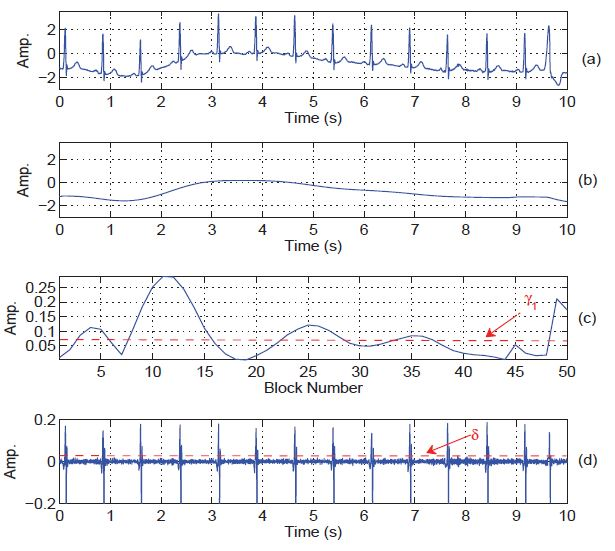
\includegraphics[width=0.55\columnwidth]{fig2.jpg}
\caption{
\wuhao
从带BW噪声ECG信号中获取的特征信号。(a)为受干扰ECG信号,(b)为提取得到的带BW噪声低频组分,(c)为动态振幅范围估计,(d)为高频组分。
}
\end{wrapfigure}
\song
该过程中,我们提出的方法使用了滑动平均滤波器来提取低频噪声组分(包含BW噪声)和高频噪声组分(包括PLI噪声,MA噪声和记录设备噪声)。滤波步骤处理了10s的ECG信号$x[n]$。用于将输入ECG信号中BW噪声(或低频噪声伪影)提取出来的滑动平均滤波器可表示如下:
\begin{equation}
  \mathbf{u}[n]=\frac{1}{L+1}\sum^{L}_{k=0}\mathbf{x}[n-k]
  \label{equ1}
\end{equation}
这里L表示滑动平均滤波器的长度。该过程中,选取这样的滤波器长度是为了让其足以捕捉到0.5Hz以下的BW噪声。同时,用于将输入ECG信号中的高频噪声(包括PLI噪声,MA噪声以及记录设备噪声)提取出来的滤波器差分方程如下:
\begin{equation}
  \mathrm{v_{1}}[n]=\frac{1}{L+1}\sum^{L}_{k=0}\mathbf{x}[n-k]
  \label{equ2}
\end{equation}

\begin{equation}
  \mathrm{v}[n]=\mathrm{x}[n]-\mathrm{v_{1}}[n],~~n=0,1,2......,N-1 
\label{equ3}
\end{equation}

第二个滑动平均滤波器长度的选取依据是令其足以捕捉40Hz以下的ECG信号。为了避免相位滞后,滤波操作采用了零相位滤波器(滤波器系数为$b_{k}=1,~~k=0,1,2,3......,L-1$)。之后,通过检测BW,PLI,MA以及记录设备噪声的出现来提取低频组分和高频组分中的噪声信号特征。图2(b)及(d)中的输出波形展示了从带噪ECG信号中获取的低频和高频组分。\\

\subsection{特征提取}
特征提取通过以下两个步骤实现:非重叠分帧和特征计算。在分帧过程中,经过滤波的信号被分为了非重叠的帧,帧长200ms。在这个过程中,信号$\mathbf{u}[n]$中第$k$帧$\mathbf{u}_{k}[n]$由以下算式给出:
\begin{equation}
  \mathbf{u}_{k}[n]=\mathbf{u}[\mathrm{P}k+n]~~n=1,2,...\mathrm{P}
  \label{equ4}
\end{equation}
此处$k=0,1...\mathrm{M}-1,\mathrm{M}=\lfloor\mathrm{\frac{N}{P}}\rfloor$,P表示帧长。通过计算每帧中振幅的最大最小值来鉴别出掩盖了PQRST波形中低振幅局域波的背景噪声。该过程中,每帧中的最大最小振幅值由如下算式计算得出:
\begin{equation}
\begin{aligned}
&a_{\max}[k]=\max \{u_{k}[n]\}~~k=0,1,...\mathrm{M-1} \\
&a_{\min}[k]=\min \{u_{k}[n]\}~~k=0,1,...\mathrm{M-1}
\end{aligned}
\label{equ5}
\end{equation}
通过比较每帧信号的动态振幅范围和预设的振幅阈值,BW噪声可以被探测到。动态振幅范围由以下算式给出:
\begin{equation}
a_{\mathrm{dr}}[k]=a_{\max}[k]-a_{\min}[k]~~k=0,1,2,...\mathrm{M}-1
 \label{equ6}
\end{equation}

特征提取中每个步骤的输出波形见图2。图2(b)中的低频组分包含了振幅出现大幅波动的BW噪声。为了将BW噪声和突变伪影区分开来,该方法估算了每帧信号的局部动态振幅范围。低频组分中,对动态振幅范围进行估算后的输出结果如图2(c)。通过设置预设的振幅阈值条件$\gamma_1,a_{\mathrm{dr}}[k]>\gamma_1$,检测得具有较低振幅帧数比率的BW噪声被与突变伪影区分开来。

\begin{table}[htbp]
\scriptsize
\centering
\caption{ECG局部波类型及其特征
\label{tabNo.1}}
\begin{tabular}{|c|c|c|}
\hline 
ECG波类型 & 振幅范围 & 持续时间 \\ 
\hline 
P波 & 0.1-0.2mV & 100ms \\ 
\hline 
QRS波群 & 0.5-1.0mV & 80-100ms \\ 
\hline 
T波 & $\approx0.5\mathrm{mV}$ & 150-200ms \\ 
\hline 
U波 & 1-2mm或T波振幅的25\% & - \\ 
\hline 
\end{tabular} 
\end{table}

对于高频噪声(如PLI和MA噪声)的检测,首先通过公式\ref{equ3}提取信号的高频组分$\mathbf{v}(n)$。滤波器的阶数被设定为能够正确捕获高频组分中50/60Hz的PLI噪声和肌电干扰噪声。以用于测试的含BW噪声ECG信号为处理对象,从中提取的高频组分如图2(d)所示。经观测,高频组分中不仅含有低振幅高频噪声,也含有部分QRS波群信号。在这一步处理过程中,通过比较高频组分振幅的最大绝对值和预设的振幅阈值$\delta$,高频噪声的影响程度得以确定。而该振幅阈值的确定则依赖于ECG信号中局部波形的各项振幅值(见表\ref{tabNo.1})。基于这些局部波振幅值,振幅阈值得以选定。低振幅的PLI噪声和肌电干扰噪声或许能通过一个简单的平滑滤波器去除。该方法假设高振幅值的PLI和肌电干扰噪声能够掩盖住中等振幅值局部波(包括P,Q,T,U波)的关键点(如起始点,终止点和峰值点)。若能使用这种噪声消除技术恢复关键点,则这时的噪声水平被认为是可接受的。振幅阈值$\delta$的选择值为0.02mV。至于高频噪声的探测,我们估算了振幅值大于$\delta=0.02\mathrm{mV}$的采样点的总数($\mathrm{N_{HF}}$)。如果估算的$\mathrm{N_{HF}>2 \times F_s}$,则算法认为存在高频噪声。

一旦确定了高频噪声确实存在,高频噪声将会被进一步分类为PLI噪声和肌电干扰噪声。
\begin{wrapfigure}{r}{24em}%靠文字内容的左侧
\label{figNo.3}
\centering
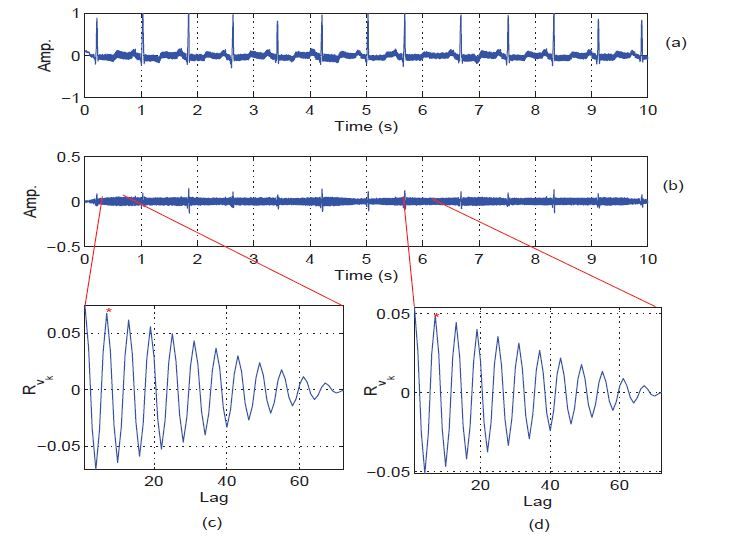
\includegraphics[width=0.5\columnwidth]{fig3.jpg}
\caption{
\wuhao
从带PLI噪声的高频组分中获取的帧信号表消除了周期性。(a)为带PLI噪声的ECG信号,(b)为提取所得带PLI噪声的高频组分仍包含了ECG中的QRS波群高频部分。(c)为第一个R峰与第二个R峰之间的采样帧中的交流信号;(d)为第八个R峰和第九个R峰之间的交流信号。
}
\end{wrapfigure}
在高频噪声分类程序中,高频组分经过了重叠分帧,帧长为200ms,帧移Q为100ms。重叠分帧的方法可表达为:
\begin{equation}
  \mathbf{v}_{k}[n]=\mathbf{v}[\frac{\mathrm{P}k}{2}+n]~~n=1,2,...\mathrm{P}
  \label{equ7}
\end{equation}
其中$k=0,1,...\mathrm{M_1}-1$,且$\mathrm{M_1}=\lfloor\frac{N}{Q}\rfloor$。在本部分处理中,利用自相关性将PLI结构噪声和肌电干扰噪声分离。在我们之前的研究中,使用自相关函数来确定信号的周期被证明是有效的。对于每帧信号$\mathbf{v}_{k}[n]$,自相关序列计算如下:
\begin{equation}
  \mathbf{R}_{k}(\tau)=\frac{1}{P}\sum^{\mathrm{P}}_{n=0}\mathbf{v}_{k}[n]\mathbf{v}_{k}[n+\tau]
  \label{equ8}
\end{equation}
其中$\mathbf{R}_{k}(\tau)$表示$\mathbf{v}_{k}[n]$的自相关函数(Autocorrelation Function, ACF),$\tau$表示自相关函数的延迟时间。通过参考第一个负过零点(由正到负的过零点称为负过零点,译者注),每帧中自相关函数的局部最大值能够被估算出来。图3表示出了自相关函数的结果,以便观察。自相关图谱显示PLI结构噪声是存在的。ACF的有效性也进一步通过处理含有肌电干扰和PLI噪声的ECG信号进行了评估。自相关性提取的输出波形见图4,图5。对于这两个带噪ECG信号,低频组分示意图显示出了振幅值小于振幅阈值$\delta$的BW噪声组分。含PLI与MA噪声的ECG信号高频组分分别见图4(d)和图5(d)。ACF特征信号见图4(e)和图5(e)。从图4(e)的ACF信号中可看出多数帧中,信号的峰值小于0.2。该实验中,我们注意到大多数帧肌电干扰信号的帧内相关性不显著。同时,图5(e)中的ACF结果显示大多数帧中的信号峰值大于0.4。通过选择一个合适的自相关峰阈值,高频组分能够被分为PLI噪声和肌电干扰噪声。一种简单的多级决策噪声检测和分类方法如图6所示。 
\begin{figure}[htbp]
\begin{center}
\begin{minipage}{0.45\linewidth}
\label{figNo.4}
\centering
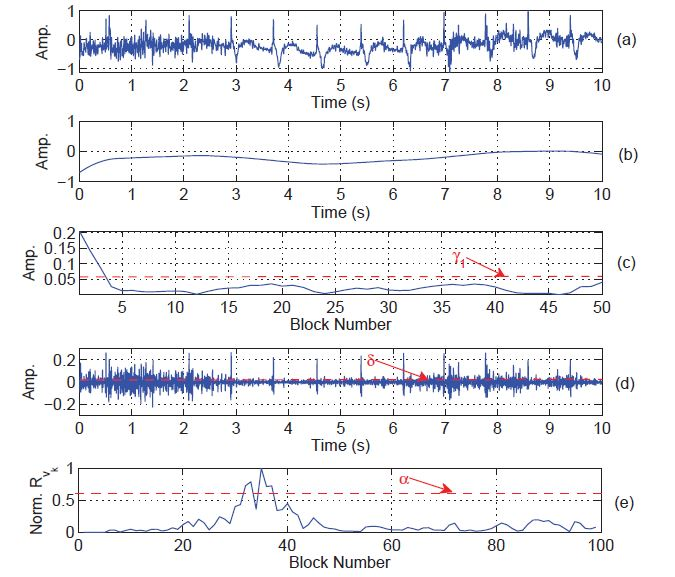
\includegraphics[height=0.8\textwidth]{fig4.jpg}
\caption{\kaishu \xiaowuhao 受肌电干扰的ECG的特征提取。(a)受干扰的ECG;(b)提取出的带BW的低频组分;(c)动态振幅范围估算;(d)高频组分;(e)最大自相关峰方法提取的自相关函数特征。}
\end{minipage}~~
\begin{minipage}{0.45\linewidth}
\label{figNo.5}
\centering
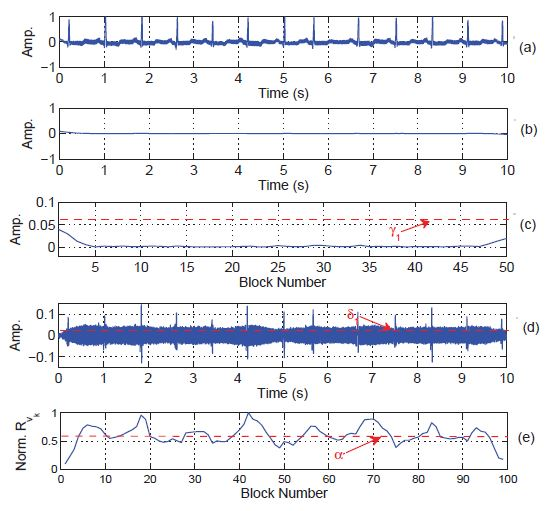
\includegraphics[height=0.8\textwidth]{fig5.jpg}
\caption{\kaishu \xiaowuhao 带PLI噪声ECG的特征提取。(a)受干扰ECG信号;(b)带BW噪声的低频组分;(c)动态振幅范围评估;(d)高频组分;(e)使用最大自相关峰提取的自相关函数特征。}

\end{minipage}
\end{center}
\end{figure}


\section{结果与讨论}

在这部分中,我们评估了所提出的噪声检测分类方法的性能,用于评测的ECG信号包含了不同形态的PQRST波,其中包括了BW噪声、ABC噪声,PLI噪声和肌电干扰噪声等多种噪声。在本研究中,第一个决策阶段首先检测了低频噪声(BW噪声和ABC噪声)和高频噪声(PLI噪声和肌电干扰噪声)是否存在。在第二个决策阶段,低频组分和高频组分被归类为BW噪声、ABC噪声,PLI噪声和肌电干扰这几类。该ECG噪声检测归类方法的简易流程图见图6。
\begin{figure}[htbp]
\label{figNo.6}
\centering
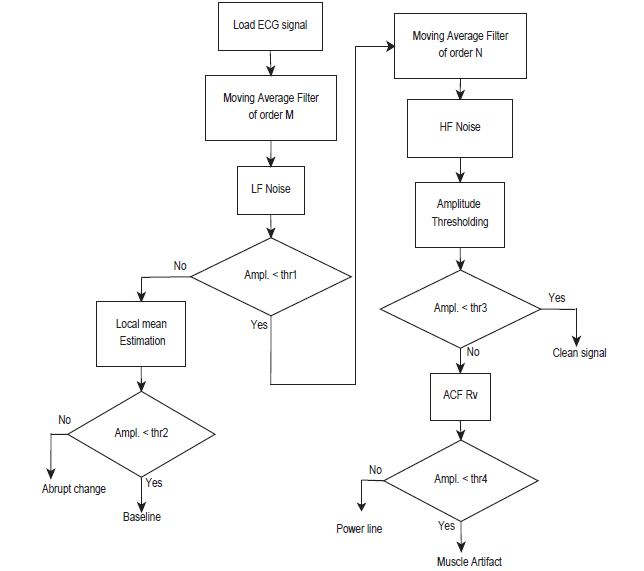
\includegraphics[width=0.7\columnwidth]{fig6.jpg}
\caption{本文中ECG噪声检测和分类方法的简易流程图
}
\end{figure}

对于性能评估方法,使用MIT-BIH心律失常数据库(MIT-BIH Arrhythmia Database, mitadb)中的ECG记录构建了大规模ECG测试信号数据库。这些ECG信号的采样率为360Hz,分辨率为11-bit。ECG测试信号数据库共含有150条ECG信号记录。每个ECG测试信号的记录时常为10s。大规模ECG测试信号数据库中的信号加入了各种不同噪声级别的噪声。这些合成的噪声通过文献21中的软件包生成。分类结果与真实数据的对比见表\ref{tab2}。

性能测试中,灵敏度Se,效率+P和精确度三种测试评分计算如下:
\begin{equation}
  Se=\frac{\mathrm{TP}}{\mathrm{TP+FN}} \times 100
  \label{equ9}
\end{equation}

\begin{equation}
  \mathrm{+P}=\frac{\mathrm{TP}}{\mathrm{TP+FP}} \times 100
  \label{equ10}
\end{equation}

\begin{equation}
  Accuracy=\frac{\mathrm{TP}}{\mathrm{TP+FN+FP}} \times 100
  \label{equ11}
\end{equation}
其中TP(True Positive)表示算法正确分类了测试片段,FP(False Positive)表示算法将测试片段错误地分为了某类噪声,FN(False Negative)表示测试片段所含的噪声类型分类错误。表\ref{tab3}总结了本文所提出方法的测试评分结果。对于大部分类型的噪声(除了ABC、PLI混合噪声以及ABC、MA混合噪声),该方法的分类准确度达到了85\%以上。表\ref{tab4}给出了本分类方法的混淆矩阵。
\begin{table}[htbp]
\scriptsize
  \centering
  \caption{噪声检测分类算法结果与真实结果比较 % 表头
  \label{tab2}}
\begin{tabular}{|c|c|c|c|c|c|c|c|c|c|}
\hline 
波形记录 & \multicolumn{9}{c|}{真实情况} \\ 
\hline 
~~ & 非带噪信号 & BW & ABC & MN & PL & BW+PL & BW+MN & ABC+PL & ABC+MN \\ 
\hline 
100 & 9 & 66 & 21 & 5 & 23 & 1 & 25 & 0 & 0 \\ 
\hline 
101 & 2 & 74 & 9 & 0 & 4 & 14 & 43 & 2 & 2 \\ 
\hline 
102 & 4 & 68 & 23 & 0 & 26 & 0 & 29 & 0 & 0 \\ 
\hline 
103 & 6 & 74 & 16 & 15 & 23 & 1 & 15 & 0 & 0 \\ 
\hline 
104 & 3 & 41 & 7 & 5 & 5 & 10 & 73 & 0 & 6 \\ 
\hline 
105 & 6 & 66 & 18 & 0 & 24 & 2 & 34 & 0 & 0 \\ 
\hline 
106 & 19 & 55 & 13 & 15 & 18 & 6 & 21 & 0 & 3 \\ 
\hline 
107 & 18 & 111 & 8 & 0 & 5 & 8 & 0 & 0 & 0 \\ 
\hline 
108 & 4 & 23 & 18 & 1 & 4 & 11 & 86 & 0 & 3 \\ 
\hline 
109 & 11 & 72 & 19 & 16 & 17 & 1 & 14 & 0 & 0 \\ 
\hline 
111 & 4 & 77 & 7 & 6 & 7 & 15 & 33 & 0 & 1 \\ 
\hline 
总数 & 86 & 727 & 159 & 63 & 156 & 69 & 373 & 2 & 15 \\ 
\hline 
波形记录 & \multicolumn{9}{c|}{算法分类结果} \\ 
\hline 
~~ & 非带噪信号 & BW & ABC & MN & PL & BW+PL & BW+MN & ABC+PL & ABC+MN \\ 
\hline 
100 & 8 & 62 & 25 & 6 & 20 & 4 & 24 & 1 & 0 \\ 
\hline 
101 & 3 & 85 & 15 & 0 & 2 & 10 & 34 & 0 & 1 \\ 
\hline 
102 & 8 & 70 & 25 & 3 & 20 & 5 & 15 & 1 & 1 \\ 
\hline 
103 & 4 & 71 & 20 & 21 & 21 & 5 & 8 & 0 & 0 \\ 
\hline 
104 & 2 & 34 & 5 & 8 & 3 & 8 & 81 & 0 & 9 \\ 
\hline 
105 & 9 & 61 & 15 & 1 & 28 & 3 & 32 & 0 & 1 \\ 
\hline 
106 & 17 & 51 & 15 & 15 & 20 & 8 & 23 & 0 & 1 \\ 
\hline 
107 & 20 & 108 & 11 & 4 & 4 & 3 & 0 & 0 & 0 \\ 
\hline 
108 & 1 & 15 & 14 & 9 & 3 & 10 & 91 & 1 & 6 \\ 
\hline 
109 & 14 & 75 & 17 & 14 & 14 & 1 & 15 & 0 & 0 \\ 
\hline 
111 & 2 & 82 & 10 & 8 & 3 & 11 & 34 & 0 & 0 \\ 
\hline 
总数 & 88 & 714 & 172 & 89 & 138 & 68 & 357 & 3 & 21 \\ 
\hline 
\end{tabular} 
\end{table}
基于表\ref{tab3}和表\ref{tab4}的结果可以认为,我们提出的方法适用于大多数常见噪声的检测,其中包括BW、PLI、ABC、MA噪声,以及BW/PLI混合噪声、BW/MA混合噪声。

\begin{table}[htp]
\scriptsize
\centering
\caption{本文中分类方法的混淆矩阵 % 表头
\label{tab4}}
\begin{tabular}{|c|c|c|c|c|c|c|c|c|c|}
\hline 
~~ & 非带噪信号 & BW & ABC & MN & PL & BW+PL & BW+MN & ABC+PL & ABC+MN \\ 
\hline 
非带噪信号 & 86 & 2 & - & - & - & - & - & - & - \\ 
\hline 
BW & 3 & 714 & - & 2 & - & - & 8 & - & - \\ 
\hline 
ABC & - & 3 & 159 & - & - & - & 6 & - & 4 \\ 
\hline 
MN & - & - & 4 & 63 & 2 & - & 14 & - & 6 \\ 
\hline 
PL & - & - & - & 7 & 138 & 9 & - & 2 & - \\ 
\hline 
BW+PL & - & - & - & - & - & 68 & 1 & - & - \\ 
\hline 
BW+MN & - & - & - & 8 & - & - & 357 & - & 8 \\ 
\hline 
ABC+PL & - & - & - & 1 & - & - & - & 2 & - \\ 
\hline 
ABC+MN & - & - & - & - & - & - & 5 & 1 & 15 \\ 
\hline 
\end{tabular} 
\end{table}
\begin{table}[htp]
\small
\centering
\caption{本文方法的分类结果 % 表头
\label{tab3}}
\begin{tabular}{|r|c|c|c|c|c|c|c|}
\hline 
信号类型 & 信号片段数量 & TP & FP & FN & Se(\%) & +P(\%) & 准确度(\%) \\ 
\hline 
非带噪信号 & 86 & 86 & 2 & - & 100 & 97.72 & 97.72 \\ 
\hline 
BW & 727 & 714 & - & 13 & 98.21 & 100 & 98.21 \\ 
\hline 
ABC & 159 & 159 & 13 & - & 100 & 92.44 & 92.44 \\ 
\hline 
MN & 63 & 63 & 26 & - & 100 & 92.44 & 92.44 \\ 
\hline 
PL & 156 & 138 & - & 18 & 88.46 & 100 & 88.46 \\ 
\hline 
BW+PL & 69 & 68 & - & 1 & 98.55 & 100 & 98.55 \\ 
\hline 
BW+MN & 373 & 357 & - & 16 & 95.71 & 100 & 95.71 \\ 
\hline 
ABC+PL & 2 & 2 & 1 & - & 100 & 66.66 & 66.66 \\ 
\hline 
ABC+MN & 15 & 15 & 6 & - & 100 & 71.42 & 71.42 \\ 
\hline 
总数 & 1650 & 1602 & 48 & 48 & 97.88 & 91.18 & 89.06 \\ 
\hline 
\end{tabular}   
\end{table}

之后,本研究将着眼于提高本文方法在检测、分类其他混合类型噪声上的性能。相较于其他现行噪声检测分类方法中的信号分离技术、特征提取技术和监督分类器,本文方法的滤波、特征提取和分类技术十分简单。而可穿戴心脏疾病监护设备由于其电量少、存储空间小、计算速率低的特点,正需要一种低复杂度的信号质量评测方法。基于我们的分类结果,我们认为本文提出的方法对于评估Holter和动态ECG信号的质量具有很高的适用性。

\section{结论}

本文提出了一种简单的ECG噪声自动检测和分类方法。这种方法由四个步骤构成:滑动平均滤波,分帧,特征提取和多级决策树算法。为了检测并分类ECG信号中的噪声,本方法提取了包括全局/局部动态振幅范围和最大自相关峰在内的信号特征。同时,本方法经过多种带噪/非带噪ECG信号输入测试并确认有效。结果表明该方法的平均灵敏度可达97.88\%,效率可达91.18\%且准确度可达89.06\%。不同于其它现行方法,本方法的滤波、特征提取和分类方法均简单易行。

\bibliographystyle{plain}
\addcontentsline{toc}{section}{参考文献}
\bibliography{Ref}
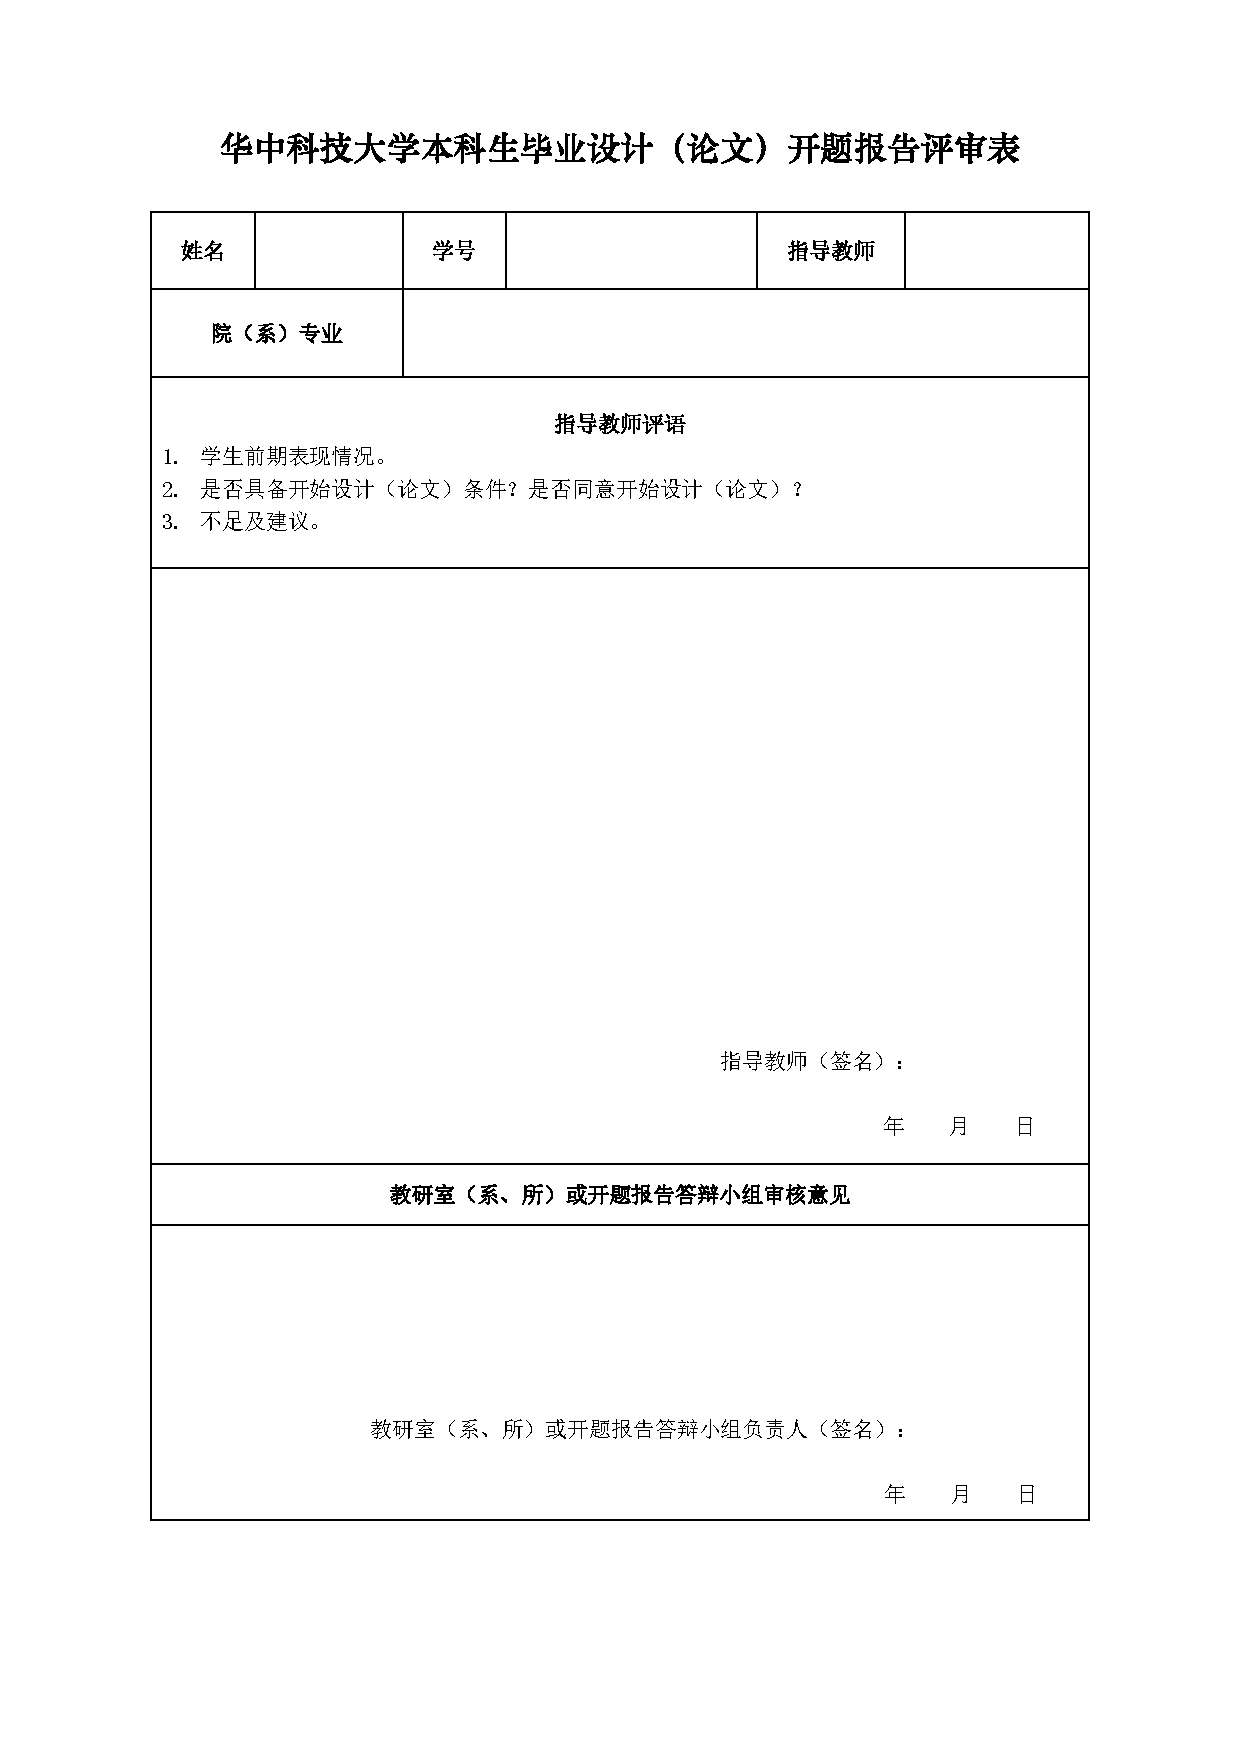
\includepdf[width=\paperwidth,pages=1]{endTable.pdf}

\end{document}
